%   Filename    : chapter_1.tex 
\chapter{Introduction}
\label{sec:researchdesc}    %labels help you reference sections of your document

\section{Overview of the Current State of Technology}
\label{sec:overview}

~~~~The Animal Welfare Act (1998), the Wildlife Resources Conservation and Protection Act (2001), and many supporting Administrative Orders govern many processes and facilities that affect animal lives in the Philippines, such as farm animal transport and pet shops. It is recommended that the Philippines' government consolidate all animal welfare legislation and jurisdictions into a single government department with adequate resources for education, enforcement, and continuing to improve animal welfare. It is also recommended that the government revise and reassess all Administrative Orders affecting animal welfare to ensure that they are in line with modern OIE standards and current scientific thinking. Furthermore, the Philippine government is strongly encouraged to prohibit cruel practices such as fur farming, keeping wild animals as pets, and long-distance animal transportation. Additional legal and policy recommendations are linked to each Animal Protection Index (API) indicator and are included in the relevant sections of this report. [1] 

Many animal rescue centers and organizations are already in place throughout the country. These animal rescue centers have their own web-based systems that allow them to operate not only physically, but also virtually. These rescue centers' web-based systems provide information about the various services they can provide to rescued animals. The systems allow for online adoption applications, cash or in-kind donations, and volunteer work at the rescue center. A vision statement, mission statement, successful projects and programs, contact information, and social media accounts are some of the information that is also provided in the system.

  
%--- the following example shows how to include a figure in PNG format
\begin{figure}[t]                %-- use [t] to place figure at top, [b] to place at the bottom, [h] for here
   \centering                    %-- use this to center the figure
   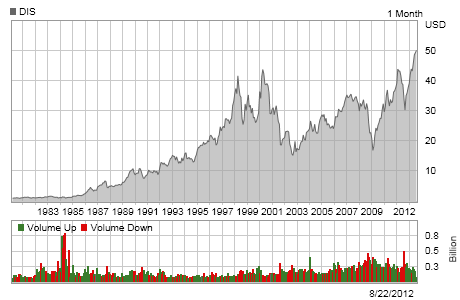
\includegraphics{DisneyChart.png}      %-- include image file named as "disneychart.png" 
   \caption{This is the figure's caption -- Disney stock chart.
   	Captions should fully describe the figure in a concise manner  such that there is not need to refer to the text when figuring out the graphic.}
    \label{fig:disneystock}
\end{figure}


Some notes on citing references.   
When using APA format, the author-date method of citation is  followed.   
This means that the author's last name and the year of publication for the source should  appear in the text, and a complete reference should appear in the reference list.

% Examples:
%     	Smith (1970) compared reaction times . . .
%     	In a recent study of reaction times (Smith, 1970), . . .   
%     	In 1970, Smith compared reaction times . . .
%	    Smith, et al., (1970) compared reaction times . . .
%     	In a recent study of reaction times (Smith, et al., 1970), . .
%     	In 1970, Smith, et al., compared reaction times . . .

Here are some examples on how to do the referencing (note author's name and years are different from commented examples).  
For APA citation details, refer to \url{http://www.ctan.org/tex-archive/biblio/bibtex/contrib/apacite/}. 

\begin{itemize}
 \item \citeA{kartch:2000:ERA} compared reaction times...
 \item In a recent study of reaction times \cite{kartch:2000:ERA}...
 \item In \citeyearNP{kartch:2000:ERA}, \citeauthor{kartch:2000:ERA} compared reaction times...
 \item \shortciteA{fedkiw:2001:VSO} compared reaction times... 
 \item In a recent study of reaction times \cite{fedkiw:2001:VSO}...
 \item In \citeyearNP{fedkiw:2001:VSO}, \shortciteauthor{fedkiw:2001:VSO}, compared reaction times...
\end{itemize}

The following are references from journal articles \cite{Park:2006:DSI, Pellacini:2005:LAH, sako:2001:SSB}.
 Here's an MS thesis document \cite{yee:2000:SSA}, and this is from PhD dissertation \cite{kartch:2000:ERA}. 
 For a book, reference is given as  \cite{parke:1996:CFA}. 
 Proceedings from a conference samples are \cite{Jobs95, fedkiw:2001:VSO, levoy:2000:TDM}.  
 The sample bibliography file named \textbf{myreferences.bib} is from the SIGGRAPH \LaTeX{}  template.  
 You can use a text editor to view the contents of the bib file.  
 It is your task to create your own bibliography file.  
 For those who downloaded papers from ACM or IEEE sites, there is a BibTeX link that you can click; thereafter, you just simply need to copy and paste the BibTeX entry into your own bibliography file.

The following shows how to include a program source code (or algorithm).  
The verbatim environment, as the name suggests, outputs text (including white spaces) as is...

\begin{verbatim}
               #include <stdio.h>
               main()
               {
                    printf("Hello world!\n");
               }
\end{verbatim}

\section{Problem Statement}

~~~~The animal rescue systems of various animal rescue centers can help in supporting Administrative Orders that govern many processes and facilities that affect animal lives in the Philippines by providing web-based systems that assist users or aspiring pet owners in looking for new homes for pets abandoned by their owners or pets separated from their family after birth.

The web-based systems currently available are user-friendly because it is simple to use, but it is not particularly interesting to users. It lacks user engagement because it only displays basic information and provides a few activities for the user to do. It is simple to use because there is no need to log in, but it does not allow you to save the transactions you generate in the system. The study aims to build a more interactive system by applying gamification and log-in features. 



\section{Research Objectives}
\label{sec:researchobjectives}

\subsection{General Objective}
\label{sec:generalobjective}

~~~~The general objective of this study is to design and develop an animal rescue system that provides better engagement between the user and the system itself.

\subsection{Specific Objectives}
\label{sec:specificobjectives}

%
%  \begin{comment} ... \end{comment} is used for multiple lines of comment
%
The specific objectives of the study are the following:

\begin{comment}
% IPR acknowledgement: the following sentences and examples are from Ethel Ong's slides 
%     on Research Objectives
How to formulate your research objectives:
1. Identify what research steps do you need to perform to achieve your general objective.
2. Identify the questions that must be answered for you to achieve your general objective.
    Thereafter, convert these questions into action statements

Example #1:

Research Question:
  What are the general features of a web-based learning environment?

Specific Objective:
   To review existing web-based learning environment that teaches language learning for children


Example #2:

Research Question:
   How will you represent commonsense knowledge for use by computer systems?

Specific Objective:
   To identify knowledge representation approaches used by existing story generation systems

Example #3:
Research Question:
   What types of storytelling knowledge are needed to generate stories?

Specific Objective:
    To identify the different types of storytelling knowledge used in generating stories

Example #4:
Research Question:
    What machine learning approaches will you utilize?

Specific Objective:
    To determine existing machine learning algorithms [that can be used in training the computer system to detect cyberbullying cases] 

Example #5: Research Question:
    How will your research output be evaluated?

Specific Objective:
    To define evaluation metrics for validating the accuracy of the translation

\end{comment}

%
%  The following are example specific objectives; replace them with your own 
%

\begin{enumerate}
   \item Implement a gamification feature in the system by having a virtual pet that monitors the transactions made by the user.
   \item Records virtual points for every activity done by the user.
   \item Apply for account creation before registering for the system.
   \item Apply automatic log-in when using the system.
\end{enumerate}


\section{Scope and Limitations of the Research}
\label{sec:scopelimitations}

~~~~The study adapts a local animal rescue center, which is the Aklan Animal Rehabilitation and Rescue Center. This study focuses on the application of gamification features to the existing system of the chosen animal rescue center and allows account creation and automatic log-in when using the system.

\begin{comment}

%
% IPR acknowledgement: the sentences inside this comment are from Ethel Ong's slides on Scope and Limitations of the Research
%
Generally, one paragraph should be allotted for each of your research objectives.

Each paragraph contains a brief overview of the concept/theory and the purpose of doing the associated objective.

Each paragraph also includes a description of the scope/limitation of your study.

* Please refer to the slides for examples.

\end{comment}


\section{Significance of the Research}
\label{sec:significance}

~~~~AKLAN ANIMAL REHABILITATION AND RESCUE CENTER. This study would help the AARRC provide better services to the public in terms of rescuing, adopting, and caring for stray animals. This will also assist the rescue center in finding more people willing to help not only these animals, but also other recipients of the funds collected by the rescue center.

AKLANON COMMUNITY. This study will help in adding a way to improve pet health in the community of Aklan. This study will assist the Aklanon community in locating an animal rescue system that will care for their rescued pets. It can also help them locate rescue organizations when they want to adopt a pet or make a donation.

PET LOVERS. This study will provide satisfaction to pet lovers who want to adopt pets not only from Aklan but also from nearby places.

COMPUTER SCIENTISTS. This study is an important step toward continuing to provide information to the public in order to promote the use of gamification features to increase the level of engagement between a user and a system.

RESEARCHERS. This study serves as baseline data to conduct better research and build new systems in the future regarding animal rescue systems. Future researchers will be given the responsibility of improving the present study.



%
% IPR acknowledgement: the following list of items are from Ethel Ong's slides on Significance of the Research
%


